\clearpage
\section{Conceptual Extensions of Cosmochrony — Particles, Quantum Phenomena, and Classical Limits}
  \label{sec:appendix-conceptual}

  This appendix develops a set of conceptual and phenomenological extensions of the
  Cosmochrony framework.
  Its purpose is not to introduce additional postulates or to strengthen the internal
  consistency of the theory, but to illustrate how familiar particle, quantum, and
  classical structures may emerge once the $\chi$ field admits localized and stable
  configurations.

  In particular, this appendix addresses:
  \begin{itemize}
    \item the ontological status of the $\chi$ field and its interpretation as a
    pre-geometric relational substrate
    (Section~\ref{subsec:nature-chi}),
    \item the description of particles as topological solitons of $\chi$, including
    explicit constructions for fermionic and bosonic configurations
    (Sections~\ref{app:topological_solitons}--\ref{subsec:4pi_soliton}),
    \item the emergence of classical limits and the interpretation of quantum-to-classical
    transitions
    (Sections~\ref{subsec:classical-limits}--\ref{subsec:status-formulation}),
    \item and perspectives on deriving particle mass spectra from the internal dynamics
    and stability properties of the $\chi$ field
    (Section~\ref{subsec:perspectives_mass_spectrum}).
  \end{itemize}

  These developments serve as a conceptual bridge between the mathematical foundations
  presented in Appendix~\ref{sec:appendix-math} and the cosmological and observational
  considerations discussed in Appendix~\ref{sec:appendix-cosmo}.
  They demonstrate how the minimal ontological assumptions of Cosmochrony can support
  a rich hierarchy of effective physical phenomena without requiring additional
  fundamental degrees of freedom.

  None of the constructions presented in this appendix are required for the logical
  coherence or internal consistency of the Cosmochrony framework.
  The core theory remains fully defined by the relational relaxation dynamics of the
  $\chi$ field.
  Rather, the material collected here illustrates how particle-like excitations,
  quantization, and classical behavior may arise naturally as emergent features when
  $\chi$ organizes into localized, topologically stable configurations.

  \subsection{Interpretative Status of the $\chi$ Field}
  \label{subsec:nature-chi}

  This subsection does not introduce new postulates regarding the $\chi$ field.
  Its purpose is purely interpretative: to clarify how $\chi$ should be understood
  \emph{once the framework has been established}, and to prevent several common
  misreadings suggested by conventional field-theoretic language.

  In the main text, $\chi$ is often written in the form $\chi(x^\mu)$ and manipulated
  using continuous differential operators.
  This notation should not be taken to imply that $\chi$ is a physical field
  propagating \emph{within} a pre-existing spacetime manifold.
  Rather, spacetime coordinates serve only as convenient labels for organizing
  relational information in regimes where a stable geometric description has emerged.

  Fundamentally, $\chi$ encodes a relational scale of relaxation from which notions
  such as duration, distance, and causal ordering are reconstructed.
  The apparent embedding of $\chi$ in spacetime is therefore representational,
  not ontological.
  The manifold description is a secondary construct, introduced only after the
  relaxation dynamics of $\chi$ has reached sufficient regularity to admit a
  geometric interpretation.

  This distinction mirrors the use of continuum variables in hydrodynamics or
  elasticity theory.
  Just as a velocity field does not exist independently of the underlying molecular
  interactions, $\chi(x^\mu)$ does not represent a fundamental spacetime field.
  It summarizes collective relational properties of the substrate once coarse
  graining becomes meaningful.

  In this sense, $\chi$ should not be interpreted as:
  \begin{itemize}
    \item a matter field living on spacetime,
    \item a dynamical scalar coupled to a pre-existing metric,
    \item or a hidden-variable replacement for the quantum wavefunction.
  \end{itemize}

  Instead, $\chi$ constitutes the pre-geometric quantity from which spacetime
  structure, effective fields, and physical observables emerge through projection
  and coarse graining.
  The use of continuous fields, Lagrangians, and differential equations throughout
  this work reflects practical representational choices rather than fundamental
  commitments.

  This interpretative clarification is particularly important for understanding the
  role of localized excitations, solitonic structures, and effective fields discussed
  in the remainder of this appendix.
  These constructions should be read as regime-dependent invariants of the underlying
  $\chi$ dynamics, not as evidence that $\chi$ itself decomposes into independently
  propagating physical entities.

  In summary, the $\chi$ field is not a field \emph{in} spacetime.
  Spacetime is an emergent bookkeeping structure \emph{for} $\chi$ once its relational
  dynamics becomes sufficiently regular.
  This asymmetry is essential to the ontological parsimony of the Cosmochrony
  framework and underlies its reinterpretation of geometry, matter, and quantum
  phenomena.

  \subsection{Topological Configurations of the \(\chi\) Field: Solitons as Particles}
  \label{app:topological_solitons}

  \paragraph{Status of this construction.}
    The solitonic configurations described in this section are not introduced as
    fundamental degrees of freedom of Cosmochrony.
    They constitute \emph{effective geometric models} intended to illustrate how
    particle-like properties may emerge from stable configurations of the $\chi$
    field once a continuum and orientable geometric description becomes applicable.

    At the fundamental level, Cosmochrony does not assume a pre-existing spatial
    manifold, metric, or differential structure.
    A fully relational formulation, free of geometric presuppositions, is presented
    separately in Appendix~\ref{app:relational_formulation}.
    The present constructions should therefore be understood as phenomenological
    representations valid in the emergent geometric regime.

  In Cosmochrony, particles are interpreted as \textbf{topologically stable solitons} of the \(\chi\) field, where their
  properties---such as \textbf{spin, charge, and mass}---emerge from the \textbf{local deformation of \(\chi\)} and its
  topological structure.
  Below, we classify these configurations and explicitly link them to particle properties, emphasizing how
  \textbf{charge arises from the modulation of \(\chi\)'s relaxation}.

  \subsubsection{Charge as Local Deformation of \(\chi\)}
    The \textbf{sign of a particle's charge} (positive or negative) is determined by how it deforms the \(\chi\)
    field:
    \begin{itemize}
      \item A \textbf{positive charge} corresponds to a \textbf{local extension of \(\chi\)} (a "peak"), which resists relaxation and repels other positive charges (as two peaks cannot merge).
      \item A \textbf{negative charge} corresponds to a \textbf{local contraction of \(\chi\)} (a "trough"), which attracts positive charges (as a peak and trough can annihilate or merge).
    \end{itemize}
    This geometric interpretation explains \textbf{Coulomb-like interactions}
    without invoking a fundamental electromagnetic field, but as a consequence of \(\chi\) dynamics.

    \begin{figure}[h]
      \centering
      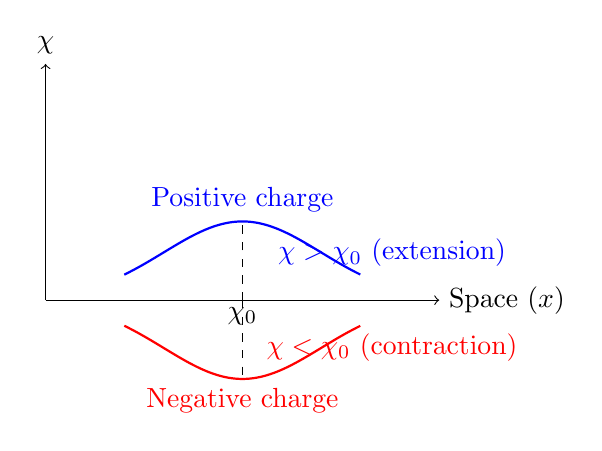
\begin{tikzpicture}[x=2cm, y=2cm]
        % Axes
        \draw[->] (0,0) -- (2.5,0) node[right] {Space (\(x\))};
        \draw[->] (0,0) -- (0,1.5) node[above] {$\chi$};
        % Positive charge: Peak in chi
        \draw[thick, blue, domain=0.5:2, samples=100] plot (\x, {0.5*exp(-2*(\x-1.25)^2)});
        \node[blue, above] at (1.25, 0.5) {Positive charge};
        \draw[dashed] (1.25,0) -- (1.25,0.5);
        \node at (1.25,-0.1) {$\chi_0$};
        % Negative charge: Trough in chi
        \draw[thick, red, domain=0.5:2, samples=100] plot (\x, {-0.5*exp(-2*(\x-1.25)^2)});
        \node[red, below] at (1.25, -0.5) {Negative charge};
        \draw[dashed] (1.25,0) -- (1.25,-0.5);
        % Labels
        \node[blue] at (2.2, 0.3) {$\chi > \chi_0$ (extension)};
        \node[red] at (2.2, -0.3) {$\chi < \chi_0$ (contraction)};
      \end{tikzpicture}
      \caption{
        Local deformations of the $\chi$ field representing positive (peak) and negative (trough) charges.
        The extension or contraction of $\chi$ relative to its background value $\chi_0$ determines the sign of the
        charge and the nature of its interactions (This figure and following ones are schematic representations intended
        to illustrate the geometric and topological structure of $chi$-field excitations, not numerical solutions of the
        dynamical equations.).
      }
      \label{fig:chi_charges}
    \end{figure}


  \subsubsection{Vortices (Charged Particles with Spin)}
    Vortices in the \(\chi\) field are characterized by a quantized winding number \(n\):
    \[
      n = \frac{1}{2\pi} \oint \nabla \arg(\chi) \cdot d\mathbf{l}.
    \]
    The \textbf{charge of the vortex} is determined by the \textbf{sign of its deformation}:
    \begin{itemize}
      \item For \(n > 0\), the vortex creates a \textbf{local extension of \(\chi\)} (positive charge).
      \item For \(n < 0\), the vortex creates a \textbf{local contraction of \(\chi\)} (negative charge).
    \end{itemize}
    The energy of the vortex scales with \(n^2\), reflecting the \textbf{mass of the particle}
    , while its winding determines the \textbf{spin} (e.g., \(n=1\) for spin-1 bosons).

    \begin{figure}[h]
      \centering
      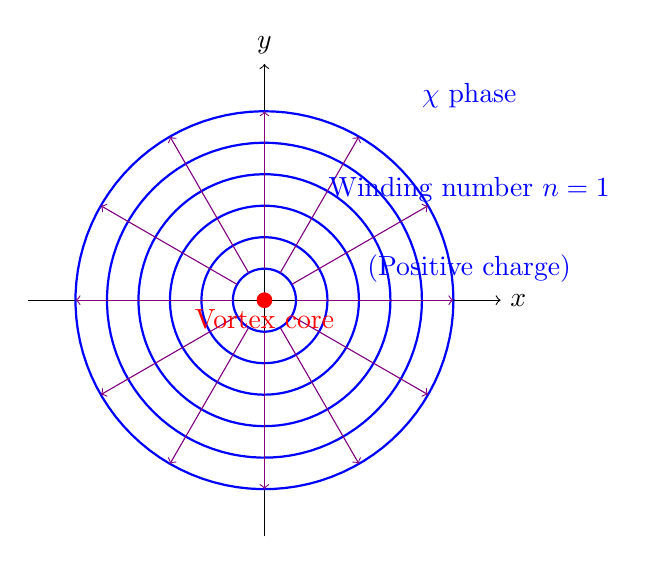
\begin{tikzpicture}[x=2cm, y=2cm]
        % Axes
        \draw[->] (-1.5,0) -- (1.5,0) node[right] {$x$};
        \draw[->] (0,-1.5) -- (0,1.5) node[above] {$y$};
        % Vortex field lines (streamlines of chi)
        \foreach \r in {0.2, 0.4, ..., 1.2} {
          \draw[blue, thick, domain=0:6.28, samples=100, variable=\t]
          plot ({\r*cos(\t r)}, {\r*sin(\t r)});
        }
        % Chi field phase (color gradient)
        \foreach \t in {0, 30, ..., 330} {
          \draw[red!50!blue, ->, domain=0.2:1.2, samples=20, variable=\r]
          plot ({\r*cos(\t)}, {\r*sin(\t)});
        }
        % Core of the vortex
        \fill[red] (0,0) circle (0.05);
        \node[red, below] at (0,0) {Vortex core};
        % Labels
        \node[blue] at (1.3, 1.3) {$\chi$ phase};
        \node[blue] at (1.3, 0.7) {Winding number $n=1$};
        \node[blue] at (1.3, 0.2) {(Positive charge)};
      \end{tikzpicture}
      \caption{
        Vortex configuration in the $\chi$ field, characterized by a winding number $n=1$.
        The circular phase gradient (arrows) represents the spin of the particle, while the core (red dot) corresponds to a localized deformation of $\chi$ (positive charge).
        Such configurations model charged bosons with quantized angular momentum.
      }
      \label{fig:chi_vortex}
    \end{figure}

  \subsubsection{Skyrmions (Fermions with Charge and Spin-1/2)}
    Skyrmions are 3D solitons with a topological charge \(Q\):
    \[
      Q = \frac{1}{4\pi} \int \mathbf{n} \cdot (\partial_x \mathbf{n} \times \partial_y \mathbf{n}) \, dx \, dy,
    \]
    where \(\mathbf{n} = \chi / |\chi|\).
    The \textbf{charge of the skyrmion} is linked to the
    \textbf{polarity of its \(\chi\) deformation}:
    \begin{itemize}
      \item A skyrmion with \(Q = +1\) and a \textbf{peak in \(\chi\)} represents a
      \textbf{positively charged fermion} (e.g., proton).
      \item A skyrmion with \(Q = -1\) and a \textbf{trough in \(\chi\)} represents a
      \textbf{negatively charged fermion} (e.g., electron).
    \end{itemize}
    The \(4\pi\)-periodicity of skyrmions under rotations explains their \textbf{spin-1/2}
    nature, while the deformation of \(\chi\) accounts for their charge.

    \begin{figure}[h]
      \centering
      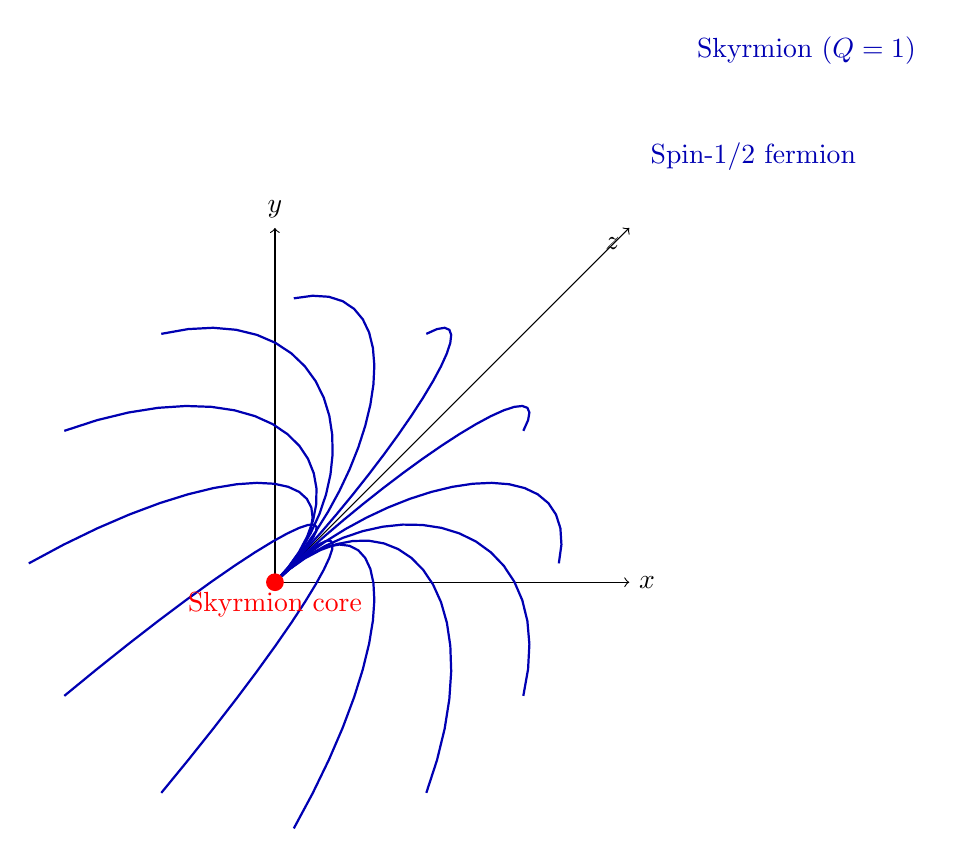
\begin{tikzpicture}[x=1.5cm, y=1.5cm, z=1.5cm, scale=1.5]
        % Axes
        \draw[->] (0,0,0) -- (2,0,0) node[right] {$x$};
        \draw[->] (0,0,0) -- (0,2,0) node[above] {$y$};
        \draw[->] (0,0,0) -- (0,0,2) node[below left] {$z$};
        % Skyrmion field (simplified representation)
        \foreach \phi in {0, 30, ..., 330} {
          \draw[blue!70!black, thick, domain=0:1.5, samples=20, variable=\r]
          plot ({\r*sin(deg(\r))*cos(\phi)}, {\r*sin(deg(\r))*sin(\phi)}, {\r*cos(deg(\r))});
        }
        % Core and labels
        \fill[red] (0,0,0) circle (0.05);
        \node[red, below] at (0,0,0) {Skyrmion core};
        \node[blue!70!black] at (1.5, 1.5, 1.5) {Skyrmion ($Q=1$)};
        \node[blue!70!black] at (1.5, 1.2, 1.2) {Spin-1/2 fermion};
      \end{tikzpicture}
      \caption{
        Skyrmion configuration in the $\chi$ field, with topological charge $Q=1$.
        The 3D structure reflects the fermionic nature of the particle (spin-1/2), where the core (red dot) represents a localized excitation of $\chi$.
        Skyrmions provide a geometric model for fermions, with their charge determined by the polarity of the $\chi$ deformation.
      }
      \label{fig:chi_skyrmion}
    \end{figure}

  \subsubsection{Summary: Topology and Charge}
    The relationship between topology and charge in Cosmochrony is summarized in ~\ref{tab:solitons_charge}

    \begin{table}[htbp]
      \centering
      \caption{Topological Solitons, Charge, and \(\chi\) Deformation}
      \label{tab:solitons_charge}
      \begin{tabular}{|c|c|c|c|}
        \hline
        \textbf{Soliton Type} & \textbf{Topological Invariant} & \textbf{\(\chi\) Deformation} &
        \textbf{Particle Property} \\
        \hline
        Vortex & Winding number \(n\) & Peak (\(n>0\)) or trough (\(n<0\)) & Charge
        \(\propto n\), spin \(\propto |n|\) \\
        Skyrmion & Charge \(Q\) & Peak (\(Q>0\)) or trough (\(Q<0\)) & Charge
        \(\propto Q\), spin-1/2 \\
        \hline
      \end{tabular}
    \end{table}

  \subsection{Soliton Energy and Structural Mass Scaling}
  \label{subsec:soliton_energy_mass}

  \paragraph{Status and scope of this analysis.}
    This subsection presents a \emph{quantitative but non-numerical} analysis of the
    effective mass associated with localized solitonic configurations arising in the
    \emph{projectable regime} of Cosmochrony.
    The objective is not to reproduce the observed particle mass spectrum, but to
    identify robust scaling relations, hierarchy constraints, and structural dependencies
    that emerge independently of microscopic details.

    No claim is made that the expressions introduced below define a fundamental
    Hamiltonian or Lagrangian for the \(\chi\) field.
    A fully predictive derivation of particle masses would require a complete effective
    theory incorporating projection dynamics, interaction channels, and renormalization
    effects, which lies beyond the scope of the present work.

    All energetic and spectral quantities discussed in this section refer exclusively
    to the effective projected field \(\chi_{\mathrm{eff}}\).
    The fundamental \(\chi\) field itself does not admit an energy functional or mass
    interpretation.

  \paragraph{Mass as integrated resistance to relaxation.}
    Within Cosmochrony, the mass of a localized excitation is interpreted as a measure of
    the total \emph{resistance to relaxation} imposed by the configuration on the
    surrounding \(\chi_{\mathrm{eff}}\) field.

    Once an effective geometric description applies, this resistance can be summarized
    by an effective diagnostic functional
    \begin{equation}
      M_{\mathrm{eff}} \;\propto\;
      \int_{\mathcal{V}}
      \left[
        \mathcal{T}\!\left(\nabla \chi_{\mathrm{eff}}\right)
        + \mathcal{U}\!\left(\chi_{\mathrm{eff}}\right)
      \right]
      \, d^3x ,
    \end{equation}
    where:
    \begin{itemize}
      \item \(\mathcal{T}\) encodes gradient-induced resistance associated with spatial
      inhomogeneities of \(\chi_{\mathrm{eff}}\),
      \item \(\mathcal{U}\) represents effective nonlinear stabilization terms arising
      from collective relaxation constraints.
    \end{itemize}

    This expression should be understood as a \emph{coarse-grained measure} of structural
    complexity rather than as a fundamental energy density.
    It quantifies how strongly a localized configuration delays or distorts the global
    relaxation of the projected field.

  \paragraph{Scaling with soliton size and internal structure.}
    Consider a localized solitonic configuration characterized by:
    \begin{itemize}
      \item a typical spatial extent \(\ell\),
      \item a characteristic deformation amplitude \(\Delta \chi_{\mathrm{eff}}\).
    \end{itemize}

    Dimensional analysis then yields the generic scaling
    \begin{equation}
      M_{\mathrm{eff}} \;\sim\;
      \ell^3
      \left[
        \frac{(\Delta \chi_{\mathrm{eff}})^2}{\ell^2}
        + V_{\mathrm{eff}}(\Delta \chi_{\mathrm{eff}})
      \right],
    \end{equation}
    where \(V_{\mathrm{eff}}\) denotes an effective nonlinear stabilization potential
    generated by projection and relaxation constraints.

    For simple kink-like configurations, the balance between gradient resistance and
    nonlinear stabilization dynamically fixes the soliton width \(\xi\).
    In this regime, the effective mass scale may be written schematically as
    \begin{equation}
      M_{\mathrm{eff}} \;\sim\;
      \sqrt{\lambda_{\mathrm{eff}}}\,\xi\,\chi_c^2 ,
    \end{equation}
    where:
    \begin{itemize}
      \item \(\chi_c\) denotes the characteristic local relaxation scale,
      \item \(\lambda_{\mathrm{eff}}\) is an emergent, configuration-dependent stiffness
      parameter.
    \end{itemize}

    Neither \(\chi_c\) nor \(\lambda_{\mathrm{eff}}\) should be interpreted as
    fundamental constants.
    They summarize collective properties of the projected relaxation regime.

  \paragraph{Structural stabilization and finite mass.}
    When stabilization arises from a balance between gradient-induced resistance and
    nonlinear relaxation constraints, the soliton size \(\ell\) is dynamically fixed.
    This mechanism ensures that localized excitations possess a finite and stable
    effective mass without the need for fine-tuning.

    Different classes of solitonic configurations (kinks, vortices, knotted or linked
    structures) involve distinct internal organizations of \(\chi_{\mathrm{eff}}\).
    As a result, their effective masses exhibit different scaling behaviors with respect
    to \(\ell\) and \(\Delta \chi_{\mathrm{eff}}\).

    This implies that mass hierarchies arise \emph{structurally} rather than through
    arbitrary parameter choices.

  \paragraph{Topological classes and mass hierarchy.}
    The effective mass depends not only on the spatial extent of a soliton but also on
    its topological class.
    Configurations characterized by higher winding, linking, or covering indices
    necessarily involve increased internal gradients and more complex relaxation
    constraints.

    Consequently, masses associated with different topological families obey ordering
    relations of the form
    \begin{equation}
      M_{n+1} \;>\; M_n ,
    \end{equation}
    where \(n\) labels an effective topological invariant.
    This establishes a natural mechanism for discrete mass hierarchies without introducing
    ad hoc mass parameters.

  \paragraph{Spectral interpretation.}
    From a spectral perspective, localized excitations correspond to bound modes of the
    linearized relaxation operator around a solitonic background configuration of
    \(\chi_{\mathrm{eff}}\).

    The effective mass is then controlled by the lowest nontrivial eigenvalue of this
    operator,
    \begin{equation}
      M_{\mathrm{eff}} \;\sim\; \lambda_{\min}^{-1},
    \end{equation}
    where \(\lambda_{\min}\) denotes the smallest positive eigenvalue governing the
    stability of the configuration.

    This formulation emphasizes that mass is fundamentally a \emph{spectral property}
    of the relaxation dynamics rather than an intrinsic attribute of a particle-like
    object.

  \paragraph{Robustness and universality.}
    The scaling relations derived above depend only on generic features of the projected
    \(\chi\) dynamics—locality, monotonic relaxation, and nonlinear stabilization—and
    are therefore expected to be robust against modifications of microscopic details.

    While specific numerical values of particle masses cannot be fixed at this level,
    the existence of discrete, ordered, and stable mass scales emerges as a structural
    prediction of the framework.

  \paragraph{Order-of-magnitude consistency.}
    Although the present analysis does not aim to reproduce the observed particle mass
    spectrum, it is instructive to examine whether the structural parameters entering the
    solitonic energy scale admit values compatible with known masses.

    For a simple kink-like configuration with characteristic width
    \(\lambda_{\mathrm{eff}}^{-1}\) and amplitude set by the local relaxation scale
    \(\chi_c\), the effective rest energy scales as
    \begin{equation}
      E_{\mathrm{sol}} \;\sim\; \chi_c^2 \lambda_{\mathrm{eff}},
    \end{equation}
    up to dimensionless shape-dependent factors of order unity.

    Identifying this energy with the electron rest mass,
    \(E_{\mathrm{sol}} \sim m_e c^2 \approx 0.511\,\mathrm{MeV}\),
    and expressing all quantities in natural units (\(\hbar = c = 1\)),
    one finds that reproducing the electron mass requires
    \begin{equation}
      \lambda_{\mathrm{eff}} \;\sim\; 10^{-44},
    \end{equation}
    for \(\chi_c\) normalized near the Planck scale.

    Such an extremely small value should not be interpreted as a fundamental coupling.
    Rather, it strongly suggests that \(\lambda_{\mathrm{eff}}\) is dynamically generated
    through collective relaxation, projection effects, and topological constraints of
    the \(\chi\) field.

  \paragraph{Summary.}
    Localized solitonic configurations of the projected field \(\chi_{\mathrm{eff}}\)
    naturally possess finite effective masses determined by their size, internal
    organization, and topological class.
    Rather than predicting specific numerical values, Cosmochrony constrains the
    \emph{scaling, ordering, and stability} of masses through geometric and spectral
    principles.

    This structural quantitativity provides a coherent foundation for future extensions
    toward a fully predictive effective theory, without compromising the pre-geometric
    nature of the fundamental \(\chi\) field.

  \subsection{Example: \(4\pi\)-Periodic Soliton and Spin-1/2}
  \label{subsec:4pi_soliton}

  To illustrate how a \(4\pi\)
  -periodic soliton can represent a spin-1/2 particle, consider a 1D soliton solution for the \(\chi\)
  field with a phase twist. Let \(\chi(x)\) be a complex field defined as:

  \[
    \chi(x) = \eta \tanh(\kappa x) e^{i \theta(x)},
  \]

  where \(\eta\) is the amplitude, \(\kappa\) determines the soliton's width, and \(\theta(x)\)
  is the phase. For a spin-1/2 particle, the phase \(\theta(x)\) must satisfy:

  \[
    \theta(x + 2\pi) = \theta(x) + \pi, \quad \theta(x + 4\pi) = \theta(x) + 2\pi.
  \]

  This \(4\pi\)-periodicity reflects the double-valuedness of spinors under rotations.

  \subsubsection{Explicit Construction of a \(4\pi\)-Periodic Soliton}

    Define the phase \(\theta(x)\) as:

    \[
      \theta(x) = \frac{x}{2},
    \]

    so that a full rotation \(x \to x + 4\pi\) returns the phase to its original value:

    \[
      \theta(x + 4\pi) = \frac{x + 4\pi}{2} = \theta(x) + 2\pi.
    \]

    The soliton solution is then:

    \[
      \chi(x) = \eta \tanh(\kappa x) e^{i x/2}.
    \]

    This soliton has the following properties:
    \begin{itemize}
      \item It is localized around \(x = 0\), with \(\chi(x) \to 0\) as \(|x| \to \infty\).
      \item The phase winds by \(\pi\) as \(x\) goes from \(-\infty\) to \(+\infty\), but a full \(2\pi\)
      rotation of the soliton requires \(x \to x + 4\pi\), reflecting the spin-1/2 nature.
    \end{itemize}

  \subsubsection{Topological Interpretation}

    The \(4\pi\)-periodicity of the soliton is a manifestation of its \textbf{topological winding number}
    . For a closed loop in space, the phase change \(\Delta \theta\) is given by:

    \[
      \Delta \theta = \oint \nabla \theta \cdot d\mathbf{l} = 2\pi n,
    \]

    where \(n\) is the winding number. For a spin-1/2 particle, the effective winding is \(n = 1/2\)
    , but since the phase must be single-valued in space, the soliton must traverse the loop twice to return to
    its original state, hence the \(4\pi\)-periodicity.

  \subsubsection{Connection to Quantum Statistics}

    The \(4\pi\)-periodicity of the soliton directly implies that it obeys \textbf{fermionic statistics}:
    \begin{itemize}
      \item Under a \(2\pi\) rotation, the wavefunction of the soliton acquires a phase of \(e^{i\pi} = -1\)
      , which is the hallmark of a fermion.
      \item This explains the \textbf{Pauli exclusion principle}
      : two identical solitons cannot occupy the same state because their wavefunctions would interfere
      destructively due to the \(-1\) phase factor.
    \end{itemize}

    \begin{figure}[h]
      \centering
      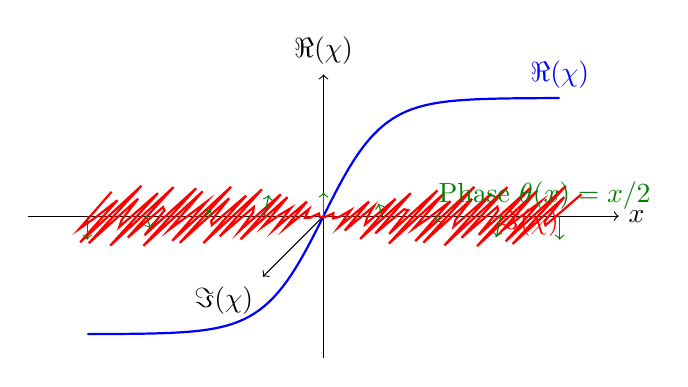
\begin{tikzpicture}[x=1.5cm, y=1.5cm]
        % Axes
        \draw[->] (-2.5,0) -- (2.5,0) node[right] {$x$};
        \draw[->] (0,-1.2) -- (0,1.2) node[above] {$\Re(\chi)$};
        \draw[->] (0,0) -- (0,0,2) node[below left] {$\Im(\chi)$};

        % Real part of chi
        \draw[thick, blue, domain=-2:2, samples=100] plot (\x, {tanh(2*\x)}, 0);
        \node[blue, above] at (2, 1, 0) {$\Re(\chi)$};

        % Imaginary part of chi
        \draw[thick, red, domain=-2:2, samples=100] plot (\x, 0, {tanh(2*\x)*sin(deg(90*\x))});
        \node[red, above] at (2, 0, 1) {$\Im(\chi)$};

        % Phase arrows
        \foreach \x in {-2, -1.5, ..., 2} {
          \pgfmathsetmacro{\phase}{90*\x}
          \draw[green!50!black, ->] (\x, 0, 0) -- (\x, {0.2*cos(\phase)}, {0.2*sin(\phase)});
        }
        \node[green!50!black] at (2, 0.3, 0.5) {Phase $\theta(x) = x/2$};
      \end{tikzpicture}
      \caption{
        Visualization of a \(4\pi\)-periodic soliton representing a spin-1/2 particle.
        The real part \(\Re(\chi)\) (blue) and imaginary part \(\Im(\chi)\) (red) of the \(\chi\) field are shown,
        along with the local phase (green arrows).
        The phase winds by \(\pi\) over the spatial extent of the soliton, but a full \(2\pi\)
        rotation of the soliton requires a \(4\pi\) change in phase, reflecting its fermionic nature.
      }
      \label{fig:4pi_soliton}
    \end{figure}

  \subsection{Relation to Classical Limits}
  \label{subsec:classical-limits}

  In Cosmochrony, the emergence of classical behavior does not correspond to the
  introduction of an independent theoretical layer.
  Instead, classical physics arises as a \emph{dynamical regime} of the same underlying
  scalar structure, characterized by smoothness, dilution of localized excitations,
  and the suppression of topological and relational effects.

  \paragraph{Weakly structured regime and effective linearization.}
    In regimes where the fundamental field \(\chi\) admits a stable projective
    representation and where its effective projection \(\chi_{\mathrm{eff}}\) varies
    slowly over large scales, localized excitations become dilute and weakly interacting.
    Under these conditions, the dynamics of \(\chi_{\mathrm{eff}}\) can be linearized
    around a quasi-homogeneous background configuration.

    In this regime, small perturbations propagate as weak disturbances on an effectively
    flat geometric background.
    Superposition, approximate locality, and linear wave propagation emerge as effective
    properties of the coarse-grained relaxation dynamics.
    This reproduces the operational content of classical field theories and of quantum
    field theories formulated on Minkowski spacetime.

    This correspondence should be understood as an \emph{effective recovery} rather than
    as an ontological reduction.
    Cosmochrony does not reduce to standard quantum field theory; rather, standard field
    theories appear as limiting descriptions valid when relational structure becomes
    dynamically inert.

  \paragraph{Suppression of relational and topological effects.}
    In the weakly structured regime, topological constraints associated with solitonic
    configurations are either absent or dynamically irrelevant.
    The configuration space effectively factorizes, and collective relaxation dominates
    over localized structural organization.
    As a result, particle-like excitations behave as approximately independent degrees
    of freedom, and classical intuition becomes applicable.

    The classical limit therefore corresponds to a regime in which the relational content
    of \(\chi\) is present but operationally inaccessible, masked by coarse-graining and
    scale separation.

  \paragraph{Nonlinear regime and effective curvature.}
    Conversely, in regimes of strong spatial variation of \(\chi_{\mathrm{eff}}\) or high
    density of localized excitations, nonlinear effects dominate the dynamics.
    Large gradients locally constrain relaxation, inducing effective curvature, time
    dilation, and horizon-like behavior in the emergent geometric description.

    These regimes reproduce the phenomenology associated with curved spacetime,
    gravitational collapse, and strong-field effects, while remaining governed by the same
    underlying scalar dynamics.
    No additional gravitational degrees of freedom are introduced; curvature emerges as
    a collective response of the relaxation structure of \(\chi_{\mathrm{eff}}\).

  \paragraph{Meaning of the classical limit in Cosmochrony.}
    The classical limit in Cosmochrony is therefore not defined by \(\hbar \to 0\), nor by
    the suppression of quantum postulates.
    It corresponds to a regime in which:
    \begin{itemize}
      \item the effective projection \(\chi_{\mathrm{eff}}\) is smooth and slowly varying,
      \item localized excitations are dilute and weakly correlated,
      \item topological and relational constraints are dynamically suppressed,
      \item coarse-graining yields stable geometric descriptions.
    \end{itemize}

    In this regime, classical spacetime and standard field dynamics emerge as reliable,
    approximate descriptions.
    Their validity reflects not fundamental structure, but the stability of a particular
    relaxation regime of the underlying \(\chi\) field.

  \subsection{Status of the Formulation}
  \label{subsec:status-formulation}

  The formulation presented in this work should be understood as a
  \emph{minimal yet structurally complete} theoretical framework.
  Its ontological commitments, dynamical principles, and interpretative structure
  are fully specified at the conceptual level, even though several technical
  developments remain open.

  In particular, a fully covariant action principle formulated solely in terms of
  the fundamental \(\chi\) dynamics, as well as a systematic quantization procedure,
  have not yet been derived in their final and definitive form.
  These missing elements should not be interpreted as conceptual deficiencies.
  Rather, they correspond to technical extensions required to interface a
  fundamentally relational and pre-geometric framework with conventional
  variational and quantum formalisms that presuppose spacetime structure.

  Crucially, the absence of a finalized action or quantization scheme does not
  obstruct the recovery of known physical phenomenology.
  Throughout this work, general relativity and quantum field theory emerge as
  \emph{effective, coarse-grained descriptions} valid within specific dynamical
  regimes of the projected field \(\chi_{\mathrm{eff}}\).
  They are not introduced as independent axioms, but arise as stable limits of the
  underlying relaxation dynamics.

  The present formulation therefore occupies a well-defined intermediate status.
  It is not intended as a closed or final theory, nor as a phenomenological model
  tuned to reproduce specific experimental data.
  Instead, it provides a coherent ontological and dynamical foundation from which
  both geometric and quantum structures can emerge, while remaining open to future
  refinements that may enhance its mathematical completeness, formal elegance, and
  predictive scope.

  In this sense, Cosmochrony should be viewed as a foundational framework rather
  than as a fully developed effective field theory: its primary contribution lies
  in clarifying \emph{what is fundamental} and \emph{how known physical structures
can arise}, rather than in prescribing their final mathematical implementation.

  \subsection{Soliton and Particle Solutions}
  \label{subsec:soliton-and-particle-solutions}

  Within the Cosmochrony framework, elementary particles are interpreted as stable
  or metastable localized configurations arising in the \emph{projectable regime}
  of the scalar field \(\chi\).
  These configurations, hereafter referred to as \(\chi\)-solitons, emerge from
  nonlinear self-organization of the relaxation dynamics and persist as localized
  resistances to global relaxation.

  This interpretation does not rely on the postulation of additional fundamental
  degrees of freedom.
  The only fundamental entity is the scalar field \(\chi\), which is not defined on
  spacetime.
  Spatial localization, energy, and particle-like persistence arise only once an
  effective geometric projection \(\chi_{\mathrm{eff}}\) becomes applicable.

  While the fundamental field is scalar, certain solitonic configurations of
  \(\chi_{\mathrm{eff}}\) possess a nontrivial internal organization that cannot be
  faithfully encoded by a single real scalar variable.
  In particular, configurations characterized by internal cyclic structure,
  nontrivial winding, and \(4\pi\)-periodicity exhibit transformation properties
  that require a double-valued representation under effective rotations.

  In such cases, an effective spinorial description becomes unavoidable.
  This does not imply the existence of fundamental spinor fields.
  Rather, spinorial variables arise as \emph{collective descriptors} encoding the
  internal topology and spectral structure of fermionic \(\chi\)-solitons.

  At the phenomenological level, these excitations admit a representation in terms
  of Dirac spinors.
  This representation should be understood as an emergent and coarse-grained
  description of the internal degrees of freedom of \(\chi\)-solitons, not as an
  ontological extension of the theory.
  Within this regime, the Dirac equation appears as the minimal effective dynamical
  structure compatible with:
  \begin{itemize}
    \item approximate locality in the projected geometric description,
    \item effective relativistic covariance,
    \item and the topological constraints associated with \(4\pi\)-periodic
    configurations.
  \end{itemize}

  From this perspective, the Dirac structure does not introduce new fundamental
  entities.
  It provides a compact and universal encoding of the internal topology, spectral
  stability, and transformation behavior of fermionic solitons.
  Spin, fermionic statistics, and exclusion behavior arise as effective consequences
  of the nontrivial configuration space of these scalar-field excitations, rather
  than as independent postulates.

  The existence and stability of \(\chi\)-solitons impose structural constraints on
  the effective self-interaction functional governing the projected dynamics.
  Although the explicit form of this functional remains undetermined, it must satisfy
  the following minimal requirements:
  \begin{enumerate}
    \item the support of localized configurations with finite effective mass,
    \item dynamical stability under small perturbations,
    \item and the existence of topologically inequivalent sectors corresponding to
    distinct classes of particle-like excitations.
  \end{enumerate}

  The detailed derivation of effective Dirac dynamics from fluctuations around
  \(\chi\)-soliton backgrounds, as well as the emergence of a realistic mass
  spectrum, remains an open mathematical problem.
  These issues are addressed at a programmatic and illustrative level in
  Sections~\ref{app:topological_solitons}--\ref{subsec:4pi_soliton} and further
  discussed in Appendix~\ref{subsec:perspectives_mass_spectrum}.

  \subsection{Perspectives: Towards a Derivation of the Proton-to-Electron Mass Ratio}
  \label{subsec:perspectives_mass_spectrum}

  The proton-to-electron mass ratio is one of the most precisely measured dimensionless quantities in physics.
  Within the Cosmochrony framework, the purpose of this section is not to derive this
  value from first principles, but to clarify how such a ratio could emerge
  \emph{structurally} from the spectral and topological organization of localized
  solitonic excitations of the projected field \(\chi_{\mathrm{eff}}\).

  The discussion should therefore be understood as a minimal and exploratory spectral ansatz.
  Its aim is to identify the relevant mechanisms, constraints, and scaling relations
  that any successful derivation would have to satisfy, rather than to provide a complete microscopic calculation.

  \subsubsection*{Spectral Stability Hypothesis}

    Let \(\chi_{\mathrm{sol}}\) denote a stationary localized configuration arising in
    the projectable regime of the \(\chi\) dynamics.
    Small perturbations \(\delta\chi_{\mathrm{eff}}\) around this background are
    governed, at the coarse-grained level, by a linear stability operator
    \(\mathcal{L}_{\mathrm{sol}}\), defined as the second variation of an effective localization functional.

    Normal modes satisfy the eigenvalue problem
    \begin{equation}
      \mathcal{L}_{\mathrm{sol}} \psi_n = \lambda_n \psi_n .
    \end{equation}

    The eigenvalues \(\lambda_n\) characterize the resistance of the soliton to
    localized deformations.
    They encode intrinsic stiffness scales associated with the internal organization
    of the solitonic configuration.

    \paragraph{Spectral mass scaling.}
      In regimes where an effective wave description applies, the normal modes exhibit
      characteristic oscillation frequencies
      \begin{equation}
        \omega_n = c \sqrt{\lambda_n} .
      \end{equation}

      Identifying the lowest nontrivial frequency with the rest energy of the excitation
      leads to the effective scaling relation
      \begin{equation}
        m_n \;\propto\; \sqrt{\lambda_n}\,\chi_c ,
      \end{equation}
      where \(\chi_c\) denotes a characteristic geometric scale associated with the
      spatial extension of the solitonic configuration in the projected regime.

      This relation does not define a fundamental mass formula.
      It provides a coarse-grained link between spectral stability and inertial mass,
      consistent with the interpretation of mass as integrated resistance to relaxation.

    \paragraph{Dimensional interpretation.}
      The eigenvalues \(\lambda_n\) carry dimensions of inverse length squared,
      reflecting the restoring stiffness of the soliton per unit deformation.
      The scale \(\chi_c\) has dimensions of length and sets the geometric extension over
      which this stiffness is distributed.

      The combination \(\lambda_n \chi_c^2\) therefore defines a characteristic energy scale,
      \begin{equation}
        E_n \sim \lambda_n \chi_c^2 ,
      \end{equation}
      which is identified with a rest energy through the effective relativistic matching \(E = mc^2\) once a spacetime
      description becomes applicable.

      This identification does not invoke a fundamental quantum constant and remains
      valid independently of the emergence of \(\hbar_{\mathrm{eff}}\).

  \subsubsection*{Projection Scale and Effective Normalization}

    The fundamental description of the \(\chi\) field is formulated in terms of
    relational relaxation rules rather than a spacetime action with fixed physical units.
    When a continuum approximation applies, an effective action for perturbations
    around a stable soliton may be introduced as a bookkeeping device.

    In this regime, the effective action for perturbations
    \(\delta\chi_{\mathrm{eff}}\) may be written schematically as
    \begin{equation}
      S_{\mathrm{eff}}[\delta\chi]
      =
      \int d^4x \,
      \frac{1}{2}
      \left( \frac{\chi_c}{c} \right)^2
      \left[
        (\partial_t \delta\chi)^2
      -
      c^2 (\nabla \delta\chi)^2
      \right] .
    \end{equation}

    Expressing this action in emergent spacetime coordinates introduces a geometric
    rescaling factor linking \(\chi\)-space and spacetime lengths.
    As a result, the canonical normalization of localized modes involves a quadratic
    scaling factor of the form
    \begin{equation}
      \left( \frac{\chi_c}{\ell_{\mathrm{spacetime}}} \right)^2 ,
    \end{equation}
    which controls the effective normalization of spectral quantities.

    This factor reflects the geometric projection from the relational \(\chi\)
        structure to emergent spacetime observables.
        It does not represent a fundamental coupling constant.

  \subsubsection*{Energy Levels from Spectral Stability}

    The discrete energy levels associated with solitonic excitations follow from the
    spectral properties of the stability operator \(\mathcal{L}_{\mathrm{sol}}\), not
    from canonical quantization.

    For a soliton labeled by \(n\), the gradient contribution to the effective energy scales as
    \begin{equation}
      E_{\mathrm{grad}}^{(n)}
      \sim
      c^2 \lambda_n \mathcal{N}_n ,
    \end{equation}
    where \(\mathcal{N}_n\) denotes a normalization factor determined by the spatial profile of the mode.

    In the spacetime-based description, this energy is identified with the rest-mass energy,
    \begin{equation}
      E_n \equiv m_n c^2 .
    \end{equation}

    The discretization of \(E_n\) arises from topological classification and spectral
    stability, not from postulated quantum operators.
    The role of \(\hbar_{\mathrm{eff}}\) appears only when matching this description to
    quantum observables.

  \subsubsection*{Elementary versus Composite Spectral Structures}

    A key distinction must be drawn between elementary and composite solitonic
    excitations.
    Elementary particles, such as leptons, are expected to correspond to topologically
    elementary solitons whose inertial mass is dominated by a single lowest stability
    eigenvalue.

    By contrast, baryonic excitations are composite configurations.
    Their mass reflects the combined contribution of several coupled stability modes
    associated with a bound structure.
    Mass ratios therefore take the schematic form
    \begin{equation}
      \frac{m_{\mathrm{comp}}}{m_{\mathrm{elem}}}
      \;\sim\;
      \frac{\sum_k \sqrt{\lambda^{(\mathrm{comp})}_k}}
      {\sqrt{\lambda^{(\mathrm{elem})}_0}} ,
    \end{equation}
    rather than the ratio of two isolated eigenvalues.

  \subsubsection*{Ansatz for the Proton as a Composite Soliton}

    As an exploratory working hypothesis, the proton is modeled as a composite solitonic excitation.
    Specifically:
    \begin{itemize}
      \item the electron corresponds to a topologically elementary soliton with a
      fundamental stability eigenvalue \(\lambda_e\),
      \item the proton corresponds to a bound configuration involving three such
      elementary solitons, supplemented by an additional collective binding mode with
      eigenvalue \(\lambda_{\mathrm{bind}}\).
    \end{itemize}

    The choice of a three-soliton composite is motivated by stability considerations
    observed in a wide class of nonlinear field theories admitting topological solitons,
    where three-body bound states often exhibit enhanced stability due to geometric
    phase locking~\cite{BattyeSutcliffe2022}.
    This choice is not derived here from a classification of \(\chi\)-soliton sectors
    and is not postulated as fundamental.

    Skyrmion models in QCD provide an instructive analogy, but no dynamical equivalence is assumed.
    The relevance of this analogy lies in the universality of topological stabilization
    mechanisms, which do not depend on the presence of a non-Abelian gauge symmetry~\cite{MantonSutcliffe2004}.

  \subsubsection*{Mass Ratio from Spectral Scaling}

    Under these assumptions, the effective eigenvalue associated with the proton may be
    written schematically as
    \begin{equation}
      \lambda_p \;\approx\; \lambda_{\mathrm{bind}} + 3\lambda_e ,
    \end{equation}
    leading to the mass ratio
    \begin{equation}
      \frac{m_p}{m_e}
      \;\approx\;
      \sqrt{\frac{\lambda_{\mathrm{bind}} + 3\lambda_e}{\lambda_e}} .
    \end{equation}

    In the binding-dominated regime \(\lambda_{\mathrm{bind}} \gg \lambda_e\), this
    reduces to
    \begin{equation}
      \frac{m_p}{m_e}
      \;\approx\;
      \sqrt{\frac{\lambda_{\mathrm{bind}}}{\lambda_e}} .
    \end{equation}

    Matching the observed ratio \(m_p/m_e \simeq 1836\) therefore imposes the spectral
    constraint
    \begin{equation}
      \frac{\lambda_{\mathrm{bind}}}{\lambda_e}
      \;\sim\; 3.4 \times 10^{6}.
    \end{equation}

    This relation is not derived here.
    It is identified as a consistency condition constraining the relative spectral
    organization of elementary and composite solitonic sectors.

    We interpret this large spectral hierarchy as defining a dimensionless
    \emph{spectral packing fraction} $\alpha$, characterizing the relative
    density of admissible stability modes in composite versus elementary
    solitonic sectors.
    Specifically, we define
    \begin{equation}
      \alpha \;\equiv\; \frac{\lambda_e}{\lambda_{\mathrm{bind}}}
      \;\sim\; 3 \times 10^{-7}.
    \end{equation}
    This quantity does not represent a coupling constant, but a structural
    measure of spectral compression induced by topological binding.

    \paragraph{Topological Interpretation of the Spectral Hierarchy}

      Although the ratio $\lambda_{\mathrm{bind}}/\lambda_e$ is introduced here as a spectral
      consistency condition, it is natural to seek a geometric or topological interpretation
      of this large hierarchy.

      In particular, the composite nature of the proton ($Q=3$) suggests that the associated
      binding modes may correspond to configurations of increased topological complexity.
      If the stability spectrum of $L_{\mathrm{sol}}$ is controlled by the effective multiplicity
      of internal configurations admitted under the non-injective projection $\Pi$,
      then $\lambda_{\mathrm{bind}}$ may be interpreted as a coarse-grained measure of the
      volume of the corresponding projection fiber.

      From this perspective, the large ratio
      $\lambda_{\mathrm{bind}}/\lambda_e \sim 10^{6}$
      reflects not an arbitrary energy scale separation, but the rapid growth of internal
      configuration space associated with topologically composite solitons.

    \paragraph{Indicative Geometric Scale}

      Although no explicit geometric or topological model is developed at this stage,
      it is useful to translate the observed spectral hierarchy into a characteristic
      dimensionless scale.

      At a purely heuristic level, one may assume that the effective spectral weight of a
      composite soliton grows quadratically with a characteristic internal scale $\chi_c$,
      so that
      \begin{equation}
        \frac{\lambda_{\mathrm{bind}}}{\lambda_e} \sim \chi_c^{2}.
      \end{equation}
      Under this assumption, the empirical constraint
      $\lambda_{\mathrm{bind}}/\lambda_e \sim 3.4 \times 10^{6}$
      corresponds to a scale of order
      \begin{equation}
        \chi_c \sim \mathcal{O}(10),
      \end{equation}
      with a representative numerical value
      \begin{equation}
        \chi_c \approx 8.3.
      \end{equation}

      Both expressions should be regarded as indicative rather than derived.
      They simply emphasize that the required spectral hierarchy corresponds to a modest
      geometric amplification, not to an extreme or finely tuned parameter choice.

  \subsubsection*{An Explicit Working Ansatz for \(V(\chi)\)}
    \label{subsec:explicit_Vchi_ansatz}

    In the present appendix, the primary driver of mass hierarchies is the spectral organization
    of the solitonic stability operator. Nevertheless, turning this program into a falsifiable
    computational scheme requires an explicit \emph{working} form for the effective potential
    \(V(\chi)\), not as a fundamental source of masses, but as a controlled perturbation that:
    (i) stabilizes localized sectors, (ii) selects admissible core amplitudes, and (iii) produces
    fine splittings within a given topological class.

    A minimal two-scale ansatz compatible with these roles is a \emph{multi-well} (or weakly periodic)
    potential with a characteristic amplitude scale \(\eta\) and stiffness scale \(\lambda\):
    \begin{equation}
      V(\chi)
      \;=\;
      \frac{\lambda}{4}\,\big(\chi^2-\eta^2\big)^2
      \;+\;
      \varepsilon\,\eta^4\Big[1-\cos\!\Big(\frac{\chi}{\eta}\Big)\Big],
      \label{eq:Vchi_multiwell_periodic}
    \end{equation}
    where \(\varepsilon \ll 1\) is a dimensionless modulation parameter.
    The first term provides a robust double-well localization mechanism; the second term introduces
    a gentle quasi-periodic micro-structure capable of generating controlled intra-sector splittings
    without reparameterizing the global mass scale.

    The interpretation in Cosmochrony is strictly \emph{effective}: the coefficients in
    Eq.~\eqref{eq:Vchi_multiwell_periodic} are not fundamental constants, but phenomenological
    descriptors of how coarse-grained projectability constraints reshape the admissible configurations
    of \(\chi_{\mathrm{eff}}\).


  \subsubsection*{Linking \((\lambda,\eta)\) to Observables Without Making Mass Fundamental}
    \label{subsec:lambda_eta_to_observables}

    The parameters \(\eta\) and \(\lambda\) are introduced only to control the \emph{shape} and
    \emph{stiffness} of admissible localized sectors in the projected description. Their observable
    imprint is therefore indirect: they enter through how they shift the stability spectrum
    \(\{\lambda_n\}\) of \(\mathcal{L}_{\mathrm{sol}}\), and how robustly a given topological sector
    remains projectable under perturbations.

    \paragraph{Dimensionless control combinations.}
      For a localized profile with characteristic extension \(\chi_c\), the potential introduces
      two natural dimensionless combinations,
    \begin{equation}
      g \;\equiv\; \lambda\,\chi_c^2\,\eta^2,
      \qquad
      u \;\equiv\; \varepsilon\,,
      \label{eq:dimensionless_controls}
      \end{equation}
      which govern (i) the curvature scale of \(V(\chi)\) near admissible minima, and (ii) the magnitude
      of sub-structure corrections. The spectral hierarchy derived above is then phrased as the statement
      that the \emph{ratio} \(m_p/m_e\) is predominantly controlled by topological/composite spectral packing,
      while \((g,u)\) control the \emph{stability} and \emph{splittings} of the low-lying spectrum.

    \paragraph{Matching strategy using the proton-to-electron ratio.}
      Denote by \(\lambda_e(g,u)\) the fundamental stability eigenvalue of the \(Q=1\) sector, and by
      \(\lambda_{\mathrm{bind}}(Q=3;g,u)\) the characteristic binding-band scale of the composite sector.
      The empirical constraint
      \(\lambda_{\mathrm{bind}}/\lambda_e \sim 3.4\times 10^6\)
      derived in Eq.~(the spectral constraint above) is then reinterpreted as a \emph{feasibility condition}:
    \begin{equation}
      \exists\,(g,u)\ \text{s.t.}\quad
      \frac{\lambda_{\mathrm{bind}}(Q=3;g,u)}{\lambda_e(g,u)}
      \;\approx\; 3.4\times 10^6,
      \label{eq:feasibility_condition_lambda_eta}
      \end{equation}
      while remaining stable under small variations of \((g,u)\).
      In other words, \((\lambda,\eta)\) are not tuned to \emph{set} the mass ratio, but to ensure that the
      \emph{topological spectral mechanism} can realize the required hierarchy in a broad basin of effective
      parameters.

    \paragraph{Secondary observables: fine splittings as diagnostics.}
      Once a viable region in \((g,u)\) exists, the same potential ansatz predicts that small
      intra-sector differences (e.g. neutron--proton splitting, excited baryonic resonances, or
      generational splittings) arise from:
    \begin{itemize}
      \item perturbative eigenvalue shifts \(\delta\lambda_n(g,u)\) induced by local curvature variations of \(V\),
      \item weak breaking of idealized symmetries in composite sectors,
      \item environment-dependent dressing of the effective coefficients through projectability constraints.
      \end{itemize}
      These effects are conceptually aligned with the claim that \(V(\chi)\) controls fine structure rather
      than the global mass scale.


  \subsubsection*{Numerical Program: From \(V(\chi)\) to Spectral Hierarchies}
    \label{subsec:numerical_program_mass_ratio}

    The numerical goal is not to simulate QCD, but to test a \emph{structural} claim:
    whether bounded relaxation dynamics plus a controlled effective potential admits stable localized
    sectors whose stability spectra exhibit (i) a robust elementary mode \(\lambda_e\), and
    (ii) a dense binding band \(\lambda_{\mathrm{bind}}\) in a composite \(Q=3\) sector, separated by a large gap.

    A minimal computational pipeline is:
    \begin{enumerate}
      \item \textbf{Dynamics and formation.} Implement the bounded relaxation update rule for \(\chi\)
      in a discretized representation (spectral/finite-element basis or lattice proxy), including
      the effective potential term Eq.~\eqref{eq:Vchi_multiwell_periodic} as a controlled perturbation.
      \item \textbf{Soliton harvesting.} Identify long-lived localized configurations and classify them
      by topological diagnostics (winding/charge proxies, knot-like invariants when available, or
      stability under deprojection/reprojection cycles).
      \item \textbf{Stability operator extraction.} For each harvested configuration, compute the
      linearized stability operator \(\mathcal{L}_{\mathrm{sol}}\) (second variation of the effective
      localization functional) and extract its low-lying eigen-spectrum.
      \item \textbf{Spectral ratio test.} Evaluate whether the emergent spectra support a regime where
      \(\lambda_{\mathrm{bind}}/\lambda_e \sim 10^6\) arises \emph{without fine tuning}, and whether the
      ratio remains stable under moderate variation of \((g,u)\).
      \item \textbf{Fine-structure diagnostics.} Measure the sensitivity of subleading splittings
      \(\delta\lambda_n\) to \((g,u)\), providing a concrete handle for how \(V(\chi)\) affects
      intra-sector structure while leaving the leading hierarchy topologically controlled.
    \end{enumerate}

    This numerical program connects directly to the broader simulation framework described in the
    technical appendix on simulation algorithms and spectral extraction, and provides a clear set of
    falsifiable diagnostics: either large, robust spectral gaps appear generically in composite sectors,
    or the proposed topological-spectral mechanism fails to reproduce the required hierarchy.

  \subsubsection*{Transition}
    The role of \(V(\chi)\) is therefore operational: it stabilizes and perturbs admissible projected sectors
    while the \emph{origin} of the mass hierarchy remains spectral and topological. This separation is
    developed further in the subsequent appendices on spectral ontology and on the secondary role of \(V(\chi)\).

  \subsection{Spectral Scaling and the Projection Ontology}
  \label{subsec:spectral-scaling-projection-ontology}

  The preceding derivation of the mass ratio $m_p/m_e$ rests on a fundamental shift in the ontology of mass.
  Within the Cosmochrony framework, inertial mass is no longer treated as an
  intrinsic ``charge'', but as a spectral signature of projection visibility.

  \paragraph{Mass as Spectral Weight}
    The non-injective nature of the projection $\Pi$ (see Section~\ref{subsec:intrinsic-structural-indeterminacy})
    implies that any effective particle in $\chi_{\mathrm{eff}}$ corresponds to a large
    equivalence class of micro-configurations in the substrate $\chi$.
    The stability eigenvalues $\lambda_n$ of the operator $L_{\mathrm{sol}}$ can
    therefore be reinterpreted as a coarse-grained measure of this structural multiplicity, or \emph{fiber weight}.
    A configuration that requires a larger set of internal modes to remain stable
    and projectable manifests a higher resistance to global relaxation, and thus a higher inertial mass.

  \paragraph{Invariance of the Ratio}
    Since the ratio
    \begin{equation}
      \frac{m_p}{m_e} \;\approx\; \sqrt{\frac{\lambda_p}{\lambda_e}}
    \end{equation}
    is independent of the absolute action scale $\hbar_\chi$, it is identified as a
    structurally protected invariant of the projection process itself.
    This explains the observed universality of the proton-to-electron mass ratio
    across cosmological epochs, regardless of the global relaxation state of $\chi$.

  \paragraph{The Spectral Packing Fraction ($\alpha$)}
    The hierarchy between the composite sector (proton) and the elementary sector
    (electron) is encapsulated by the spectral packing fraction
    \begin{equation}
      \alpha \;\equiv\; \frac{\lambda_e}{\lambda_{\mathrm{bind}}}
      \;\approx\; 3 \times 10^{-7}.
    \end{equation}
    Rather than an empirical fit, $\alpha$ represents the ratio of spectral
    transmittance under $\Pi$.
    The proton is heavy because its non-trivial topology ($Q=3$) constrains the
    stability operator $L_{\mathrm{sol}}$ to exhibit a large internal spectral bandwidth.
    This topological constraint, often heuristically represented by a trefoil-knot
    configuration, leads to a strong spectral gap between the binding modes
    $\lambda_{\mathrm{bind}}$ and the fundamental electronic mode $\lambda_e$.

  \paragraph{Conclusion}
    While the precise numerical value $m_p/m_e \simeq 1836$ awaits a closed-form
    derivation from the spectral geometry of $L_{\mathrm{sol}}$ on topologically
    constrained manifolds, the Cosmochrony framework reformulates the mass-ratio
    problem in structural terms.
    The proton-to-electron mass ratio emerges as the macroscopic signature of a
    spectral gap dictated by the complexity of the substrate’s excitations under
    projection, as schematically illustrated in Fig.~\ref{fig:spectral-gap},
    rather than as an arbitrary fundamental constant.

    \begin{figure}[htbp]
      \centering
      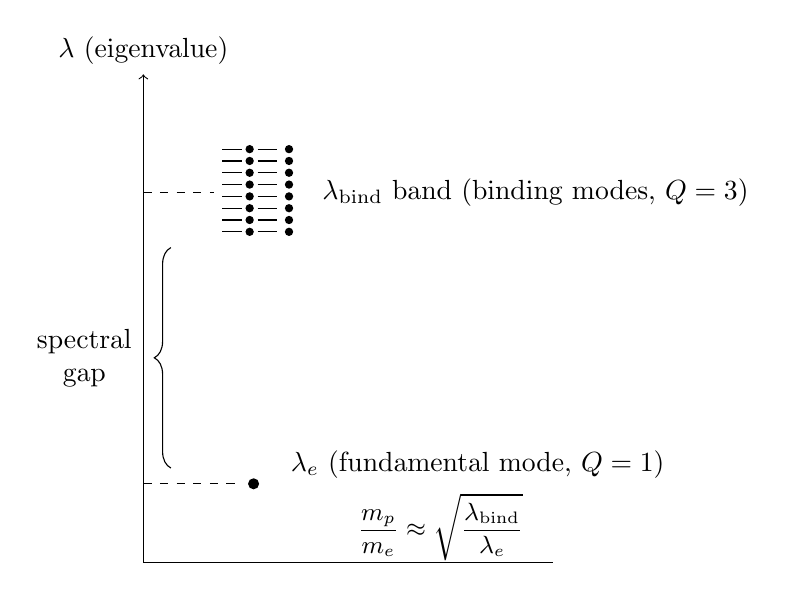
\begin{tikzpicture}[x=1cm,y=1cm]
      % Axis
      \draw[->] (0,0) -- (0,6.2) node[above] {$\lambda$ (eigenvalue)};
      \draw (0,0) -- (5.2,0);

      % Electron fundamental mode lambda_e
      \fill (1.4,1.0) circle (2pt);
      \node[anchor=west] at (1.75,1.25) {$\lambda_e$ (fundamental mode, $Q=1$)};

      % Binding band near lambda_bind
      \foreach \y in {4.2,4.35,4.5,4.65,4.8,4.95,5.1,5.25} {
        \draw (1.0,\y) -- (1.25,\y);
        \fill (1.35,\y) circle (1.5pt);
        \draw (1.45,\y) -- (1.70,\y);
        \fill (1.85,\y) circle (1.5pt);
      }
      \node[anchor=west] at (2.15,4.7) {$\lambda_{\mathrm{bind}}$ band (binding modes, $Q=3$)};

      % Indicate the gap with a brace
      \draw[decorate,decoration={brace,amplitude=6pt}]
      (0.35,1.2) -- (0.35,4.0)
      node[midway,xshift=-1.1cm,align=center] {spectral\\gap};

      % Optional dashed guide lines
      \draw[dashed] (0,1.0) -- (1.2,1.0);
      \draw[dashed] (0,4.7) -- (0.9,4.7);

      % Formula moved to the bottom-right (no overlap)
      \node[anchor=west,align=left] at (2.6,0.45)
        {\small $\displaystyle \frac{m_p}{m_e}\approx \sqrt{\frac{\lambda_{\mathrm{bind}}}{\lambda_e}}$};
    \end{tikzpicture}
    \caption{%
      Conceptual schematic of a spectral gap in the stability spectrum of
      $\mathcal{L}_{\mathrm{sol}}$.
      The elementary mode $\lambda_e$ is separated from a dense band of binding modes
      near $\lambda_{\mathrm{bind}}$, illustrating the interpretation of
      $m_p/m_e$ as a macroscopic signature of spectral organization rather than an
      intrinsic mass parameter.}
    \label{fig:spectral-gap}
\end{figure}

\subsubsection*{Summary and Outlook}

  Within the Cosmochrony framework, the proton-to-electron mass ratio is interpreted
  as an emergent constraint on the spectral and topological organization of solitonic
  excitations, not as a fundamental input parameter.

  The analysis presented here provides a coherent toy model identifying the
  conditions under which such a ratio could arise.
  Whether the required spectral hierarchy can be generated dynamically from the
  \(\chi\) relaxation dynamics remains an open problem, to be addressed through
  future analytical and numerical investigations.

  \subsection{Spectral Characterization of Mass and the Secondary Role of \(V(\chi)\)}
  \label{subsec:spectral_mass}

  This appendix clarifies the conceptual status of inertial mass in the Cosmochrony
  framework.
  Physically, mass originates from the resistance of localized configurations to the
  relaxation of the fundamental \(\chi\) field.
  This resistance, however, admits a quantitative and structurally organized
  description in terms of the spectral properties of an associated stability
  operator defined in the projectable regime.

  Spectral analysis therefore does not redefine the physical origin of inertial mass.
  Rather, it provides a coherent and potentially calculable characterization of how
  resistance to relaxation is distributed among stable and metastable configurations.

  A central conjecture of Cosmochrony is that particle masses are not fundamental
  parameters encoded in the nonlinear potential \(V(\chi)\).
  Instead, they emerge as spectral properties of a background-independent relaxation
  operator defined on a relational substrate, which may be represented, for
  calculational purposes, by a discrete graph structure.

  \paragraph{Mass spectrum as eigenmodes of a relaxation operator.}

    Localized particle-like excitations are identified with normal modes of an
    effective relaxation operator \(\Delta_G^{(0)}\), which may be represented as a
    Laplace--Beltrami operator acting on a graph \(G(V,E)\),
    \begin{equation}
      \Delta_G^{(0)} \psi_n = -\lambda_n \psi_n .
    \end{equation}
    The eigenmodes \(\psi_n\) characterize the stability of localized solitonic
    configurations, while the eigenvalues \(\lambda_n\) encode their intrinsic
    resistance to deformation.

    In regimes where an effective spacetime description applies, the inertial masses
    associated with these modes scale as
    \begin{equation}
      m_n c^2 \;\propto\; \sqrt{\lambda_n}\,\chi_c ,
    \end{equation}
    in agreement with the spectral relations introduced in
    Section~\ref{subsec:perspectives_mass_spectrum}.
    This scaling reflects the fact that inertial mass measures the characteristic
    frequency associated with the resistance of a localized configuration to
    \(\chi\)-field relaxation.

    The situation is analogous to bounded elastic systems, where discrete vibrational
    frequencies arise from geometry and connectivity rather than from adjustable
    material parameters.
    Within Cosmochrony, mass hierarchies are therefore interpreted as geometric and
    topological properties of the underlying relational structure.

    A decisive test of this conjecture would consist in computing the low-lying
    spectrum of \(\Delta_G^{(0)}\) on large but finite networks with physically
    motivated connectivity rules.
    Even approximate agreement with observed mass ratios would strongly support the
    spectral origin of inertial mass and the non-fundamental role of \(V(\chi)\).

  \paragraph{Separation of descriptive levels.}

    To avoid circular dependencies between geometry, dynamics, and emergent particle
    properties, Cosmochrony distinguishes three conceptual levels.

    At the fundamental level, inertial masses are associated with the spectral
    properties of a background-independent relaxation operator
    \(\Delta_G^{(0)}\), defined solely by the intrinsic relational connectivity of the
    substrate.
    This operator is not tied to any spacetime geometry or instantaneous \(\chi\)
    configuration and provides a stable spectral backbone.

    At the emergent geometric level, coarse-grained configurations of
    \(\chi_{\mathrm{eff}}\) give rise to effective notions of spacetime, including
    curvature, gravitational time dilation, and cosmological expansion.
    These geometric effects influence propagation and interaction, but do not redefine
    the underlying spectral operator responsible for mass generation.

    Finally, fast dynamical processes such as radiation, scattering, and decoherence
    correspond to interaction-induced redistributions of relaxation potential within
    the \(\chi\) field.
    These processes affect observables without modifying the fundamental spectral
    structure.

  \paragraph{Residual role of the potential \(V(\chi)\).}

    Within this spectral picture, the nonlinear potential \(V(\chi)\) plays a
    secondary and effective role.
    It does not set the overall mass scale.
    Instead, it provides a local coarse-grained description of nonlinear stabilization
    mechanisms associated with low-lying spectral modes.

    The admissible form of \(V(\chi)\) is constrained by the requirement that it
    support stable solitonic configurations compatible with the pre-existing spectral
    structure.
    It encodes neither an independent interaction nor a fundamental energy density.

  \paragraph{Origin of the effective potential \(V(\chi)\).}

    Characterizing \(V(\chi)\) as secondary does not imply arbitrariness.
    Rather, \(V(\chi)\) should be understood as an effective descriptor of the local
    nonlinear response of the relaxation dynamics in the vicinity of a stable
    configuration.

    At the fundamental level, the dynamics of \(\chi\) are governed by bounded
    relaxation rules and their associated spectral structure.
    When this dynamics is projected onto a reduced functional subspace associated with
    a localized soliton, nonlinear self-consistency constraints induce an effective
    local restoring structure.
    In this reduced description, these constraints may be summarized by an effective
    potential \(V(\chi)\).

    Different admissible forms of \(V(\chi)\) correspond to different coarse-graining
    choices, while leaving invariant the underlying spectral origin of mass and
    stability.

  \paragraph{Potential-induced corrections to stability eigenvalues.}

    To illustrate how \(V(\chi)\) can modify stability eigenvalues without altering
    their spectral origin, consider the illustrative form
    \begin{equation}
      V(\chi) = \lambda \left( \chi^2 - \chi_c^2 \right)^2 .
    \end{equation}

    Expanding around the relaxed background \(\chi=\chi_c\) yields a quadratic
    contribution for small fluctuations \(\delta\chi\),
    \begin{equation}
      V(\chi_c + \delta\chi)
      \simeq
      \frac{1}{2}
      \left.
        \frac{d^2 V}{d\chi^2}
      \right|_{\chi_c}
      (\delta\chi)^2 + \cdots ,
    \end{equation}
    with
    \begin{equation}
      \left.
        \frac{d^2 V}{d\chi^2}
      \right|_{\chi_c}
      \propto \lambda\,\chi_c^2 .
    \end{equation}

    This term contributes additively to the linearized stability operator, shifting the
    eigenvalues as
    \begin{equation}
      \lambda_n
      \;\longrightarrow\;
      \lambda_n^{(0)} + \Delta\lambda_n^{(V)} .
    \end{equation}

    For composite solitons, such corrections may differ slightly between closely
    related configurations (e.g., neutron versus proton), generating small mass
    splittings.
    By contrast, ratios dominated by topological organization (such as
    \(m_p/m_e\)) remain largely insensitive to the detailed form of \(V(\chi)\).

  \paragraph{Summary.}

    In Cosmochrony, inertial mass is fundamentally a spectral property of the
    relaxation dynamics of the \(\chi\) field.
    The potential \(V(\chi)\) serves as a derived, effective descriptor controlling
    fine structure, not as a primary source of mass.
    Extending this spectral characterization toward quantitative mass predictions
    requires specifying the relaxation operator and its boundary conditions,
    particularly for composite solitonic sectors.

  \subsection{Spectral Stability and the Emergence of \(\hbar_{\mathrm{eff}}\)}
\label{sec:hbar_eff_derivation}

In Cosmochrony, the effective Planck constant \(\hbar_{\mathrm{eff}}\) is not
introduced as a fundamental quantum postulate.
Instead, it emerges as a scaling parameter linking spectral stability of
\(\chi\)-field solitons to effective spacetime observables.

\subsubsection*{Fundamental scales of the \(\chi\) dynamics}

  The \(\chi\) field is characterized by three independent dynamical scales:
  \begin{itemize}
    \item \(K_0\): maximal relaxation stiffness, with dimensions \([L^{-2}]\),
    \item \(\chi_c\): correlation length at which solitonic configurations stabilize,
    \item \(c\): maximal relaxation speed.
  \end{itemize}

  From these, one may define a natural unit of action associated with the relaxation
  dynamics,
  \begin{equation}
    \hbar_{\chi}
    \;\equiv\;
    \frac{c^3}{K_0 \chi_c} ,
  \end{equation}
  which has the dimensions of action and is independent of the standard Planck
  constant.

\subsubsection*{Spectral origin of effective quantization}

  Quantization in Cosmochrony follows from the discrete spectrum of the stability
  operator \(\Delta_G^{(0)}\).
  For a solitonic excitation with eigenvalue \(\lambda_n\), the characteristic
  frequency of small oscillations scales as
  \begin{equation}
    \nu_n \;\sim\; \frac{c}{\chi_c}\,\sqrt{\lambda_n}\,\mathcal{N}_n^{1/2} .
  \end{equation}

  Identifying the rest energy with the product of this frequency and an effective
  action scale yields
  \begin{equation}
    E_n = \hbar_{\mathrm{eff}}\,\nu_n ,
  \end{equation}
  from which \(\hbar_{\mathrm{eff}}\) emerges as a geometric and spectral quantity,
  not as an independent constant.

\subsubsection*{Regime-dependent scaling}

  The effective value of \(\hbar_{\mathrm{eff}}\) depends on the scale at which the
  system is probed.
  In regimes where the characteristic spacetime scale
  \(\ell_{\mathrm{spacetime}}\) is comparable to \(\chi_c\),
  \begin{equation}
    \hbar_{\mathrm{eff}} \approx \hbar_{\chi} ,
  \end{equation}
  recovering standard quantum behavior.

  At macroscopic scales \(\ell_{\mathrm{spacetime}} \gg \chi_c\),
  \begin{equation}
    \hbar_{\mathrm{eff}}
    \approx
    \hbar_{\chi}
    \left( \frac{\chi_c}{\ell_{\mathrm{spacetime}}} \right)^2 ,
  \end{equation}
  leading to a strong suppression of quantum effects and the emergence of classical
  behavior.

\subsubsection*{Consistency with quantum phenomenology}

  In the microscopic regime, where \(\hbar_{\mathrm{eff}} \approx \hbar\), standard
  quantization relations
  \(E = \hbar \nu\) are recovered as effective descriptions.
  This agreement is not postulated but follows from the scaling behavior of
  \(\hbar_{\mathrm{eff}}\) once the projected regime matches laboratory scales.

  \paragraph{Numerical constraints.}

    Reproducing particle-scale quantum behavior requires
    \begin{equation}
      K_0 \chi_c^2 \sim \hbar ,
    \end{equation}
    which constrains the admissible values of the relaxation stiffness and correlation
    length.
    These constraints are consistent with soliton stability and do not require fine
    tuning.

  \paragraph{Summary.}

    Within Cosmochrony, both inertial mass and effective quantization emerge from the
    same spectral stability structure of the \(\chi\) relaxation dynamics.
    The Planck constant appears not as a fundamental input, but as a scale-dependent
    parameter encoding the projection from relational dynamics to spacetime-based
    observables.

  \input{B-appendix-conceptual/B12-renormalization}
  \subsection{Structural Origin of Quantum Correlations and Non-Locality}
  \label{app:structural-origin-quantum-correlations}

  This section provides a conceptual extension of the Cosmochrony framework,
  illustrating how quantum correlations and spin may be interpreted geometrically
  within a strictly monistic and non-injective projection ontology.
  The discussion is interpretative in nature and does not introduce additional
  dynamical postulates.

  The non-injective nature of the projection operator $\Pi$, which maps the relational substrate $\chi$
      onto the effective 4D manifold, provides a structural reinterpretation of quantum non-locality and entanglement.
      In this framework, EPR-type correlations are not viewed as the result of superluminal signaling, but as a direct
      consequence of the \textbf{shared ontological source} of projected observables.

  \subsubsection*{Non-injectivity and Structural Identity.}
    Within Cosmochrony, what is effectively perceived as two spatially separated particles may correspond to a single,
    unified relational configuration in $\chi$.
    \begin{itemize}
      \item \textbf{Geometric Separation vs. Relational Unity:} While the emergent metric $g_{\mu\nu}$
      assigns a large spatial distance between two detectors, the underlying $\chi$
      -excitation remains a single connected entity in the pre-geometric substrate.
      \item \textbf{The Shared Projection:} Entanglement is thus defined as the manifestation of a single $\chi$
      -source through multiple, non-injective projective ``images''.
      The perceived ``spooky action at a distance'' is an artifact of the metric description, which fails to capture the
      \item underlying relational unity.
    \end{itemize}

  \subsubsection*{Torsional Conservation and the Origin of Spin Correlations.}
    This hypothesis extends naturally to the geometric origin of spin.
    If spin is interpreted as the projection of the internal degrees of freedom of the relational fiber
    (e.g., within the Hopf fibration $S^3 \to S^2$), then:
    \begin{itemize}
      \item A measurement at location $A$ corresponds to a local stabilization of the projection's torsional phase.
      \item Because the underlying configuration in $\chi$ is a unified structure, this local stabilization
      \textit{structurally constrains} the admissible projective states available at any other location $B$
      originating from the same source.
      \item This mechanism ensures the conservation of global topological invariants across the shared projection
      without violating the causal bounds of the relaxation dynamics.
    \end{itemize}

  \subsubsection*{Relationship with Bell's Theorem.}
    Cosmochrony addresses the constraints of Bell's theorem by shifting the locus of reality. The framework remains
        \textbf{realistic}, as the substrate $\chi$ possesses definite relational states, but it is
        \textbf{structurally non-local} with respect to the emergent spacetime.
    The violation of Bell inequalities is not seen as a failure of realism, but as a signature of
        \textbf{metric emergence}
        : the metric distance, used to define ``locality'' in the theorem, is not a fundamental property of the level
        where the correlations are established.

